\documentclass[a4paper,12pt]{article}
\usepackage{amsmath}
\usepackage{amssymb}
\usepackage[polish]{babel}
\usepackage{polski}
\usepackage[utf8]{inputenc}
\usepackage{indentfirst}
\usepackage{geometry}
\usepackage{array}
\usepackage[pdftex]{color,graphicx}
\usepackage{subfigure}
\usepackage{afterpage}
\usepackage{setspace}
\usepackage{color}
\usepackage{wrapfig}
\usepackage{listings}
\usepackage{datetime}


\renewcommand{\onehalfspacing}{\setstretch{1.6}}

\geometry{tmargin=2.5cm,bmargin=2.5cm,lmargin=2.5cm,rmargin=2.5cm}
\setlength{\parindent}{1cm}
\setlength{\parskip}{0mm}

\newenvironment{lista}{
\begin{itemize}
  \setlength{\itemsep}{1pt}
  \setlength{\parskip}{0pt}
  \setlength{\parsep}{0pt}
}{\end{itemize}}

\newcommand{\linia}{\rule{\linewidth}{0.4mm}}

\definecolor{lbcolor}{rgb}{0.95,0.95,0.95}
\lstset{
    backgroundcolor=\color{lbcolor},
    tabsize=4,
  language=C++,
  captionpos=b,
  tabsize=3,
  frame=lines,
  numbers=left,
  numberstyle=\tiny,
  numbersep=5pt,
  breaklines=true,
  showstringspaces=false,
  basicstyle=\footnotesize,
  identifierstyle=\color{magenta},
  keywordstyle=\color[rgb]{0,0,1},
  commentstyle=\color{Darkgreen},
  stringstyle=\color{red}
  }
\begin{document}

\noindent
\begin{tabular}{|c|p{11cm}|c|} \hline 
Grupa 1 & Kamil Sacha, Konrad Szwedo & \ddmmyyyydate\today \tabularnewline
\hline 
\end{tabular}

\renewcommand{\lstlistingname}{Listing kodu}

\section*{Zadanie 1 - Mnożenie macierzy OpenMP}

Naszym zadaniem laboratoryjnym było napisanie współbieżnego programu, który miał obliczyć iloczyn dwóch macierzy wstępnie wypełnionymi liczbami według wzorów podanych w zadaniu. Głównym celem było stworzenia rozwiązania które miało pokazywać wpływ tworzenia oprogramowania na szybkość obliczeń.

\begin{lstlisting}[caption=Główna pętla programu - mnożenie macierzy, label=kodzik]
#pragma omp parallel for private(i, j, k) firstprivate(matrixSize) num_threads(threadCount)
for ( i = 0; i < matrixSize; i++) {
	for ( k = 0; k < matrixSize; k++) {
		for ( j = 0; j < matrixSize; j++) {
			C[i][j] += A[i][k] * B[k][j];
		}
	}
}
\end{lstlisting}

Do zrównoleglenia mnożenia macierzy została wykorzystana dyrektywa 
\textbf{omp parallel for},
która to dzięki wykorzystaniu  dyrektywy pomocniczej \textbf{num\_threads()} 
dzieli równomiernie operacje iteracji pomiędzy dostępnymi wątkami. 
Wykorzystując dyrektywę \textbf{firstprivate()} określamy, że zmienna 
\textit{matrixsize} ma zostać zainicjowana przed użyciem jej przez wątek oraz ma służyć jako zmienna prywatna, oznacza to, że każdy wątek pracuje na swojej kopii tej zmiennej.

\section*{Wyniki}

\begin{wrapfigure}{l}{0.6\textwidth}
	\vbox{-10pt}
	\resizebox{1.0\linewidth}{!}{% GNUPLOT: LaTeX picture with Postscript
\begingroup
  \makeatletter
  \providecommand\color[2][]{%
    \GenericError{(gnuplot) \space\space\space\@spaces}{%
      Package color not loaded in conjunction with
      terminal option `colourtext'%
    }{See the gnuplot documentation for explanation.%
    }{Either use 'blacktext' in gnuplot or load the package
      color.sty in LaTeX.}%
    \renewcommand\color[2][]{}%
  }%
  \providecommand\includegraphics[2][]{%
    \GenericError{(gnuplot) \space\space\space\@spaces}{%
      Package graphicx or graphics not loaded%
    }{See the gnuplot documentation for explanation.%
    }{The gnuplot epslatex terminal needs graphicx.sty or graphics.sty.}%
    \renewcommand\includegraphics[2][]{}%
  }%
  \providecommand\rotatebox[2]{#2}%
  \@ifundefined{ifGPcolor}{%
    \newif\ifGPcolor
    \GPcolortrue
  }{}%
  \@ifundefined{ifGPblacktext}{%
    \newif\ifGPblacktext
    \GPblacktextfalse
  }{}%
  % define a \g@addto@macro without @ in the name:
  \let\gplgaddtomacro\g@addto@macro
  % define empty templates for all commands taking text:
  \gdef\gplbacktext{}%
  \gdef\gplfronttext{}%
  \makeatother
  \ifGPblacktext
    % no textcolor at all
    \def\colorrgb#1{}%
    \def\colorgray#1{}%
  \else
    % gray or color?
    \ifGPcolor
      \def\colorrgb#1{\color[rgb]{#1}}%
      \def\colorgray#1{\color[gray]{#1}}%
      \expandafter\def\csname LTw\endcsname{\color{white}}%
      \expandafter\def\csname LTb\endcsname{\color{black}}%
      \expandafter\def\csname LTa\endcsname{\color{black}}%
      \expandafter\def\csname LT0\endcsname{\color[rgb]{1,0,0}}%
      \expandafter\def\csname LT1\endcsname{\color[rgb]{0,1,0}}%
      \expandafter\def\csname LT2\endcsname{\color[rgb]{0,0,1}}%
      \expandafter\def\csname LT3\endcsname{\color[rgb]{1,0,1}}%
      \expandafter\def\csname LT4\endcsname{\color[rgb]{0,1,1}}%
      \expandafter\def\csname LT5\endcsname{\color[rgb]{1,1,0}}%
      \expandafter\def\csname LT6\endcsname{\color[rgb]{0,0,0}}%
      \expandafter\def\csname LT7\endcsname{\color[rgb]{1,0.3,0}}%
      \expandafter\def\csname LT8\endcsname{\color[rgb]{0.5,0.5,0.5}}%
    \else
      % gray
      \def\colorrgb#1{\color{black}}%
      \def\colorgray#1{\color[gray]{#1}}%
      \expandafter\def\csname LTw\endcsname{\color{white}}%
      \expandafter\def\csname LTb\endcsname{\color{black}}%
      \expandafter\def\csname LTa\endcsname{\color{black}}%
      \expandafter\def\csname LT0\endcsname{\color{black}}%
      \expandafter\def\csname LT1\endcsname{\color{black}}%
      \expandafter\def\csname LT2\endcsname{\color{black}}%
      \expandafter\def\csname LT3\endcsname{\color{black}}%
      \expandafter\def\csname LT4\endcsname{\color{black}}%
      \expandafter\def\csname LT5\endcsname{\color{black}}%
      \expandafter\def\csname LT6\endcsname{\color{black}}%
      \expandafter\def\csname LT7\endcsname{\color{black}}%
      \expandafter\def\csname LT8\endcsname{\color{black}}%
    \fi
  \fi
  \setlength{\unitlength}{0.0500bp}%
  \begin{picture}(7200.00,5040.00)%
    \gplgaddtomacro\gplbacktext{%
      \csname LTb\endcsname%
      \put(1078,704){\makebox(0,0)[r]{\strut{} 1000}}%
      \csname LTb\endcsname%
      \put(1078,1111){\makebox(0,0)[r]{\strut{} 1500}}%
      \csname LTb\endcsname%
      \put(1078,1518){\makebox(0,0)[r]{\strut{} 2000}}%
      \csname LTb\endcsname%
      \put(1078,1925){\makebox(0,0)[r]{\strut{} 2500}}%
      \csname LTb\endcsname%
      \put(1078,2332){\makebox(0,0)[r]{\strut{} 3000}}%
      \csname LTb\endcsname%
      \put(1078,2740){\makebox(0,0)[r]{\strut{} 3500}}%
      \csname LTb\endcsname%
      \put(1078,3147){\makebox(0,0)[r]{\strut{} 4000}}%
      \csname LTb\endcsname%
      \put(1078,3554){\makebox(0,0)[r]{\strut{} 4500}}%
      \csname LTb\endcsname%
      \put(1078,3961){\makebox(0,0)[r]{\strut{} 5000}}%
      \csname LTb\endcsname%
      \put(1078,4368){\makebox(0,0)[r]{\strut{} 5500}}%
      \csname LTb\endcsname%
      \put(1078,4775){\makebox(0,0)[r]{\strut{} 6000}}%
      \csname LTb\endcsname%
      \put(1210,484){\makebox(0,0){\strut{} 0}}%
      \csname LTb\endcsname%
      \put(1909,484){\makebox(0,0){\strut{} 2}}%
      \csname LTb\endcsname%
      \put(2608,484){\makebox(0,0){\strut{} 4}}%
      \csname LTb\endcsname%
      \put(3307,484){\makebox(0,0){\strut{} 6}}%
      \csname LTb\endcsname%
      \put(4007,484){\makebox(0,0){\strut{} 8}}%
      \csname LTb\endcsname%
      \put(4706,484){\makebox(0,0){\strut{} 10}}%
      \csname LTb\endcsname%
      \put(5405,484){\makebox(0,0){\strut{} 12}}%
      \csname LTb\endcsname%
      \put(6104,484){\makebox(0,0){\strut{} 14}}%
      \csname LTb\endcsname%
      \put(6803,484){\makebox(0,0){\strut{} 16}}%
      \put(176,2739){\rotatebox{-270}{\makebox(0,0){\strut{}Średni czas wykonania [ms]}}}%
      \put(4006,154){\makebox(0,0){\strut{}Ilość wątków}}%
    }%
    \gplgaddtomacro\gplfronttext{%
      \csname LTb\endcsname%
      \put(5816,4602){\makebox(0,0)[r]{\strut{}Czas wykonania}}%
    }%
    \gplbacktext
    \put(0,0){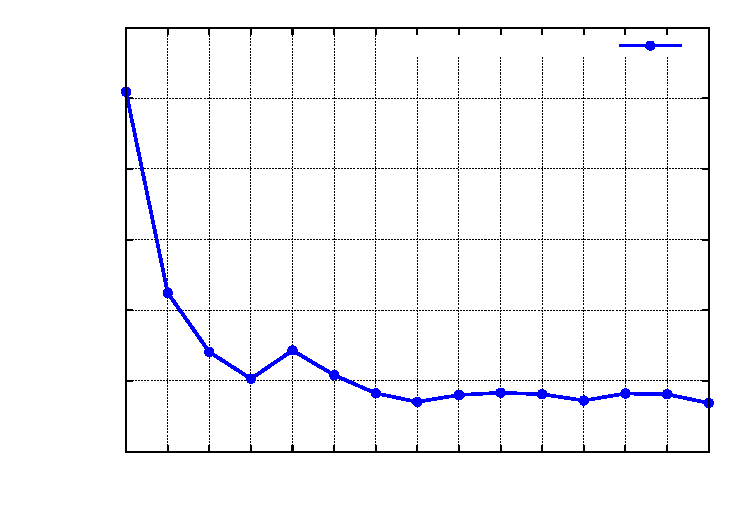
\includegraphics{wykres_czasu}}%
    \gplfronttext
  \end{picture}%
\endgroup
}    
    \caption{Wykres zależności czasu wykonania od liczby wątków. Dla rozmiaru $10^6$ danych 	macierzy.}
\end{wrapfigure}

Program za pomocą biblioteki openMP zrównoleglony został poprawnie,
o czym świadczy wykres 1. \\
Niewielkie załamanie liniowości wykresu związane jest najprawdopodobniej z wykorzystywaniem technologi \textit{HyperThreading}. 
Inną przyczyną może być też testowanie na serwerze który nie pracuje tylko i wyłącznie dla nas (wykonuje on też swoje zadania co wpływa na wynik, nie mamy 100\% dostępu do czasu procesora. 
\clearpage
\textit{Jaki wpływ na zrównoleglenie będzie miało zastosowanie poniższej dyrektywy OpenMP}

Dla pierwszej dyrektywy uzyskujemy wolniejsze zrównoleglenie ponieważ wszystkie zmienne są współdzielone. 

\begin{lstlisting}
	#pragma omp parallel for default(shared)
\end{lstlisting}
\textit{a jaki dyrektywa}

\begin{lstlisting}
#pragma omp parallel for default(none) shared(A, B, C) firstprivate(rozmiar)private(i, j)
\end{lstlisting}


\begin{wrapfigure}{r}{0.6\textwidth}
	\vspace{-10pt}
	\resizebox{1.0\linewidth}{!}{% GNUPLOT: LaTeX picture with Postscript
\begingroup
  \makeatletter
  \providecommand\color[2][]{%
    \GenericError{(gnuplot) \space\space\space\@spaces}{%
      Package color not loaded in conjunction with
      terminal option `colourtext'%
    }{See the gnuplot documentation for explanation.%
    }{Either use 'blacktext' in gnuplot or load the package
      color.sty in LaTeX.}%
    \renewcommand\color[2][]{}%
  }%
  \providecommand\includegraphics[2][]{%
    \GenericError{(gnuplot) \space\space\space\@spaces}{%
      Package graphicx or graphics not loaded%
    }{See the gnuplot documentation for explanation.%
    }{The gnuplot epslatex terminal needs graphicx.sty or graphics.sty.}%
    \renewcommand\includegraphics[2][]{}%
  }%
  \providecommand\rotatebox[2]{#2}%
  \@ifundefined{ifGPcolor}{%
    \newif\ifGPcolor
    \GPcolortrue
  }{}%
  \@ifundefined{ifGPblacktext}{%
    \newif\ifGPblacktext
    \GPblacktextfalse
  }{}%
  % define a \g@addto@macro without @ in the name:
  \let\gplgaddtomacro\g@addto@macro
  % define empty templates for all commands taking text:
  \gdef\gplbacktext{}%
  \gdef\gplfronttext{}%
  \makeatother
  \ifGPblacktext
    % no textcolor at all
    \def\colorrgb#1{}%
    \def\colorgray#1{}%
  \else
    % gray or color?
    \ifGPcolor
      \def\colorrgb#1{\color[rgb]{#1}}%
      \def\colorgray#1{\color[gray]{#1}}%
      \expandafter\def\csname LTw\endcsname{\color{white}}%
      \expandafter\def\csname LTb\endcsname{\color{black}}%
      \expandafter\def\csname LTa\endcsname{\color{black}}%
      \expandafter\def\csname LT0\endcsname{\color[rgb]{1,0,0}}%
      \expandafter\def\csname LT1\endcsname{\color[rgb]{0,1,0}}%
      \expandafter\def\csname LT2\endcsname{\color[rgb]{0,0,1}}%
      \expandafter\def\csname LT3\endcsname{\color[rgb]{1,0,1}}%
      \expandafter\def\csname LT4\endcsname{\color[rgb]{0,1,1}}%
      \expandafter\def\csname LT5\endcsname{\color[rgb]{1,1,0}}%
      \expandafter\def\csname LT6\endcsname{\color[rgb]{0,0,0}}%
      \expandafter\def\csname LT7\endcsname{\color[rgb]{1,0.3,0}}%
      \expandafter\def\csname LT8\endcsname{\color[rgb]{0.5,0.5,0.5}}%
    \else
      % gray
      \def\colorrgb#1{\color{black}}%
      \def\colorgray#1{\color[gray]{#1}}%
      \expandafter\def\csname LTw\endcsname{\color{white}}%
      \expandafter\def\csname LTb\endcsname{\color{black}}%
      \expandafter\def\csname LTa\endcsname{\color{black}}%
      \expandafter\def\csname LT0\endcsname{\color{black}}%
      \expandafter\def\csname LT1\endcsname{\color{black}}%
      \expandafter\def\csname LT2\endcsname{\color{black}}%
      \expandafter\def\csname LT3\endcsname{\color{black}}%
      \expandafter\def\csname LT4\endcsname{\color{black}}%
      \expandafter\def\csname LT5\endcsname{\color{black}}%
      \expandafter\def\csname LT6\endcsname{\color{black}}%
      \expandafter\def\csname LT7\endcsname{\color{black}}%
      \expandafter\def\csname LT8\endcsname{\color{black}}%
    \fi
  \fi
  \setlength{\unitlength}{0.0500bp}%
  \begin{picture}(7200.00,5040.00)%
    \gplgaddtomacro\gplbacktext{%
      \csname LTb\endcsname%
      \put(682,704){\makebox(0,0)[r]{\strut{} 0}}%
      \csname LTb\endcsname%
      \put(682,1722){\makebox(0,0)[r]{\strut{} 1}}%
      \csname LTb\endcsname%
      \put(682,2740){\makebox(0,0)[r]{\strut{} 2}}%
      \csname LTb\endcsname%
      \put(682,3757){\makebox(0,0)[r]{\strut{} 3}}%
      \csname LTb\endcsname%
      \put(682,4775){\makebox(0,0)[r]{\strut{} 4}}%
      \csname LTb\endcsname%
      \put(814,484){\makebox(0,0){\strut{} 1}}%
      \csname LTb\endcsname%
      \put(1242,484){\makebox(0,0){\strut{} 2}}%
      \csname LTb\endcsname%
      \put(1670,484){\makebox(0,0){\strut{} 3}}%
      \csname LTb\endcsname%
      \put(2097,484){\makebox(0,0){\strut{} 4}}%
      \csname LTb\endcsname%
      \put(2525,484){\makebox(0,0){\strut{} 5}}%
      \csname LTb\endcsname%
      \put(2953,484){\makebox(0,0){\strut{} 6}}%
      \csname LTb\endcsname%
      \put(3381,484){\makebox(0,0){\strut{} 7}}%
      \csname LTb\endcsname%
      \put(3809,484){\makebox(0,0){\strut{} 8}}%
      \csname LTb\endcsname%
      \put(4236,484){\makebox(0,0){\strut{} 9}}%
      \csname LTb\endcsname%
      \put(4664,484){\makebox(0,0){\strut{} 10}}%
      \csname LTb\endcsname%
      \put(5092,484){\makebox(0,0){\strut{} 11}}%
      \csname LTb\endcsname%
      \put(5520,484){\makebox(0,0){\strut{} 12}}%
      \csname LTb\endcsname%
      \put(5947,484){\makebox(0,0){\strut{} 13}}%
      \csname LTb\endcsname%
      \put(6375,484){\makebox(0,0){\strut{} 14}}%
      \csname LTb\endcsname%
      \put(6803,484){\makebox(0,0){\strut{} 15}}%
      \put(176,2739){\rotatebox{-270}{\makebox(0,0){\strut{}Średnie przyśpieszenie}}}%
      \put(3808,154){\makebox(0,0){\strut{}Liczba wątków}}%
    }%
    \gplgaddtomacro\gplfronttext{%
      \csname LTb\endcsname%
      \put(5816,877){\makebox(0,0)[r]{\strut{}Przyśpieszenie}}%
    }%
    \gplbacktext
    \put(0,0){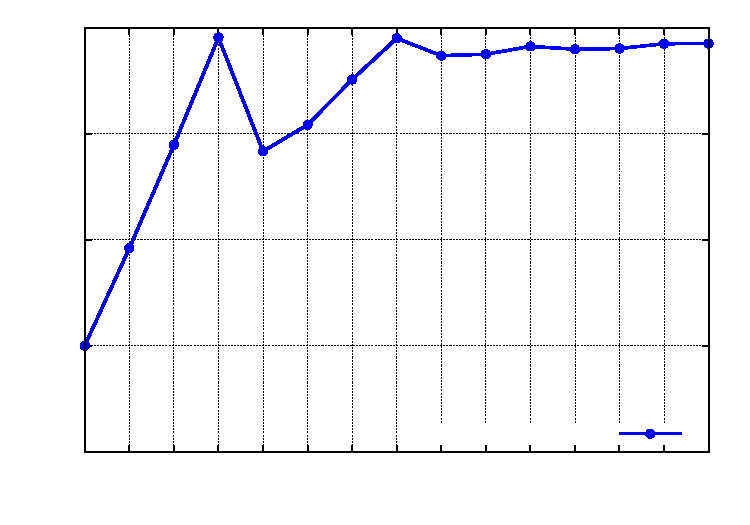
\includegraphics{dane/wykres_przyspieszenia}}%
    \gplfronttext
  \end{picture}%
\endgroup
} 	
    \caption{Wykres zależności przyśpieszenia od liczby wątków. Dla rozmiaru $10^6$ danych macierzy.}
\end{wrapfigure}


Największą wydajność uzyskujemy dla 4 wątków, naszym zdaniem związane jest to z tym, że w takim układzie każdy rdzeń procesora dostaje swój wątek i wykorzystuje go maksymalnie. \\


\section*{Procedura testowania}

Do przetestowania planowanego wzrostu wydajności został napisany skrypt pracujący pod powłoką BASH. Dla zadanego rozmiaru macierzy  w naszym przypadku $10^6$ oblicza średnią z 10 uruchomień naszego programu macierzomp (jako rozmiar macierzy przyjmujemy całkowitą ilość elementów jednej macierzy, wynika z tego, że macierz jest jest rozmiaru n x n gdzie n = $\sqrt[]{matrixSize}$, n jest zawsze liczbą całkowitą). W Ostatnim etapie generowany jest wykres w programie gnuplot. Program kompiluje się poprawnie poprzez kompilator \textit{g++} z flagą \textit{-O3} w celu optymalizacji kodu i tym samym przyśpieszenia wykonania programu.

\section*{Wnioski}

Jak możemy zauważyć skalowalność czasowa jest liniowa do wartości 4 wątków. Wiążę się to z kilkoma czynnikami, jednym z czynników jest to, że dla większej ilości wątków powstaje narzut współbieżności związany z tworzeniem, synchronizacją, i zarządzaniem poszczególnymi wątkami. 

Innym naszym zdaniem istotnym czynnikiem jest to, że program testowany był na serwerze pod adresem: cuda.iti.pk.edu.pl gdzie pracuje Intel\textsuperscript{\textregistered} Core\texttrademark{ }
 I7-950. Procesor ten wyposażony jest w 4 rdzenie fizyczne, które wraz z technologią 
Hyper-Threading tworzą 8 procesorów wirtualnych (widzianych dla systemu jako 8 procesorów fizycznych). Według informacji z portali zajmujących się testowaniem sprzętu, całkowity zysk ze stosowania tej technologi jest podawany jako maksymalnie 10 - 30\%. Dlatego też nie uzyskujemy skalowania liniowego rozpatrując czas wykonania dla powyżej 4 wątków.

\end{document}